% Created 2024-08-29 Thu 00:31
% Intended LaTeX compiler: pdflatex
\documentclass[11pt]{article}
\usepackage[utf8]{inputenc}
\usepackage[T1]{fontenc}
\usepackage{graphicx}
\usepackage{grffile}
\usepackage{longtable}
\usepackage{wrapfig}
\usepackage{rotating}
\usepackage[normalem]{ulem}
\usepackage{amsmath}
\usepackage{textcomp}
\usepackage{amssymb}
\usepackage{capt-of}
\usepackage{hyperref}
\date{\today}
\title{Martin Brignall}
\hypersetup{
 pdfauthor={Docker image runner},
 pdftitle={Martin Brignall},
 pdfkeywords={},
 pdfsubject={},
 pdfcreator={Emacs 27.1 (Org mode 9.3)}, 
 pdflang={English}}
\begin{document}

\maketitle
\begin{center}
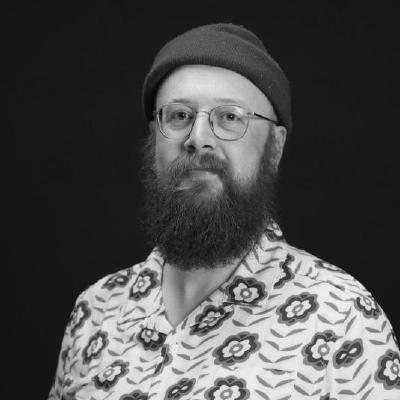
\includegraphics[width=.9\linewidth]{./img/mbrignl.jpeg}
\end{center}
\begin{center}
󰊫 \href{mailto:martinaloysiusbrignall@gmail.com}{email}  | 󰊤 \href{https://github.com/mbrignall}{github}  | 󰄜 07766027602 

\texttt{112 Aubrey Road, Bristol, BS3 3EU}
\end{center}

\section*{ABOUT ME}
\label{sec:org6bc39fc}

Over the past 5 years, I have honed my skills in the DevOps/DevSecOps space. I currently
work as a Cyber Defence Engineer as escalated Incident Response. We deal with reports/alerts
as broad as phishing/business email compromise to GuardDuty alerting or malware. I have a strong
interest in the software developement pipeline. I love learning, and use self development to
increase my understanding.

\section*{EXPERIENCE}
\label{sec:org79ad842}

\subsection*{\textbf{OVO Energy}, Bristol - Cyber Defence Engineer}
\label{sec:orgbdbbe98}
\texttt{May 2024 to Present}
\begin{itemize}
\item Building a bond between ticketing system of our MSSP and OVO (saving 30k)
\item Working with leading technologies in SOC/Threat Detection/SIEM
\begin{itemize}
\item Google Chronicle/Workspace/SecOps
\item Sublime Email Security
\item CrowdStrike
\item GuardDuty
\item Tines (Security Automation)
\item Wiz
\end{itemize}
\item Escalated Incident Response (Blue Team)
\end{itemize}

\subsection*{\textbf{OVO Energy}, Bristol - Developer Tooling Specialist}
\label{sec:orgd889d8b}
\texttt{August 2022 - May 2024}
\begin{itemize}
\item Cloud services optimization (AWS, Google Cloud) for
scalability, reliability, and targeted cost reduction
\item Building automated vending for GCP projects as guardrails
\item Drive DevOps and DevEx practices, streamlining development
workflows, and facilitating seamless collaboration between
development and operations teams
\item Champion collaboration and knowledge sharing within the
engineering community
\item Vendor engagement and billing/cost reconciliation
\end{itemize}

\subsection*{OVO Energy, Bristol - Enterprise Technology Specialist}
\label{sec:orgca11b26}
\texttt{March 2021 - August 2022}
\begin{itemize}
\item Jira Cloud Administration for all Atlassian products
\item Introduced zero-touch deployment using Mosyle, a pioneering MDM
tool for Apple devices
\item Linux device management solution including device scripting
\end{itemize}

\subsection*{OVO Energy, Bristol - Tech Support Analyst}
\label{sec:org762edde}
\texttt{June 2019 - August 2022}
\begin{itemize}
\item Provided technical support and automated Jira projects for
enhanced productivity
\item Service Desk - Front Line Support
\item Covid Office Cover
\end{itemize}

\section*{INTERESTS/SKILLS}
\label{sec:org6567f06}
\begin{itemize}
\item Home Lab | Proxmox | Containers (Docker)
\item WebDev | Django | Python
\item Terraform | Cloudflare
\item NixOS | Linux | Emacs
\item AWS | GCP | Postgres
\end{itemize}

For the last two years I've been managing a website that supports
the \href{https://sundaymarket.marketmanager.app}{Tobacco Factory Sunday Market}. This was the perfect opportunity
to hone my web development skills and I chose to use Django/Python,
home served using Proxmox and served to the web with Cloudflare. From
here I began to approach my own CI/CD and automated deployments to
better understand how best to apply these practices.

\section*{TRAINING}
\label{sec:org363ed52}
\begin{itemize}
\item Webdev Bootcamp
\item AWS Developer
\item Jira fundamentals and Atlassian University
\item Google Labs/ Security Foundations
\item Immersive Labs
\item ACE Community Leader
\end{itemize}
\end{document}
